\section{Methodology}

Building on our observation that perplexity filtering may concentrate benchmark-overlapping content, we design a methodology to measure and validate curation-contamination relationships. Our approach combines three components: contamination detection to identify benchmark-related training examples, data attribution to quantify their contribution to performance, and controlled curation experiments to establish causality.

\subsection{Problem Formulation}

Let $D$ be a training corpus and $B$ a benchmark dataset. A filtering strategy $f: D \rightarrow D_f$ selects a subset for training. We define contamination detection $c: D \times B \rightarrow \{0, 1\}$ that labels each example as contaminated (overlapping with $B$) or clean.

Given a model $M$ trained on $D_f$, let $\alpha_i^B$ denote the attribution score of training example $i$ for benchmark performance (computed via TRAK). The \textbf{Contamination Contribution Ratio} is:

\begin{equation}
\text{CCR}(M, D_f, B) = \frac{\sum_{i: c(d_i, B)=1} \alpha_i^B}{\sum_{i} \alpha_i^B}
\end{equation}

CCR measures the fraction of benchmark-attributed influence originating from contaminated examples. Higher CCR indicates greater reliance on contaminated content for benchmark performance.

\subsection{Contamination Detection via N-gram Overlap}

We detect contamination using 8-gram overlap between training documents and benchmark questions, following ConTAM recommendations that $n > 8$ leads to false negatives while $n < 8$ produces excessive false positives.

\textbf{Rationale:} While sophisticated membership inference methods (Min-K\%++, CDD) exist, n-gram detection offers interpretability and precise localization. For our purpose of quantifying curation effects, we need to identify \textit{which} training documents contain benchmark material, not just whether the model memorized it.

For document $d$ and benchmark item $b$, contamination is detected when:
\begin{equation}
c(d, b) = \mathbb{1}[\exists \text{ 8-gram } g : g \in d \land g \in b]
\end{equation}

This binary signal feeds into CCR computation by identifying the contamination-flagged subset.

\subsection{Attribution via TRAK}

We compute attribution scores using TRAK (Attributing Model Behavior at Scale), which approximates influence functions through random projection. TRAK expresses the counterfactual effect of removing example $i$ on benchmark performance as:

\begin{equation}
\alpha_i^B \approx \nabla_\theta \mathcal{L}_B(\theta)^\top H^{-1} \nabla_\theta \mathcal{L}_i(\theta)
\end{equation}

where $H$ is the Hessian approximated via random projection matrices $P \in \mathbb{R}^{k \times p}$:

\begin{equation}
\alpha_i^B \approx (P \nabla_\theta \mathcal{L}_B(\theta))^\top (P \nabla_\theta \mathcal{L}_i(\theta))
\end{equation}

\textbf{Rationale:} TRAK scales to billion-parameter models with validated precision ($\sim$70\% in counterfactual studies). We compute benchmark-specific attribution by aggregating over benchmark examples.

\subsection{Experimental Design: Matched Corpus Comparison}

To isolate filtering strategy effects from corpus composition confounds, we use a matched corpus design:

\begin{enumerate}
    \item \textbf{Single source corpus}: RedPajama-V2 (English, snapshot 2023-14)
    \item \textbf{Three filtering strategies} applied to the same source:
    \begin{itemize}
        \item \textit{Perplexity-filtered}: Bottom 30\% by \texttt{ccnet\_perplexity} (low perplexity = high quality per Wikipedia LM)
        \item \textit{Random-sampled}: Uniform random selection
        \item \textit{Inverse-perplexity}: Top 30\% by perplexity (control condition)
    \end{itemize}
    \item \textbf{Matched token budget}: $\sim$1B tokens per strategy
    \item \textbf{Multiple seeds}: 5 random seeds per strategy for variance estimation
\end{enumerate}

\textbf{Rationale:} Using pre-computed perplexity scores from RedPajama-V2 ensures our filtering matches production pipelines. The matched corpus design isolates filtering effects from corpus-level confounds.

\subsection{CCR Validation via Synthetic Injection}

Before comparing strategies, we validate CCR as a reliable metric through synthetic contamination injection:

\begin{enumerate}
    \item Inject MMLU test questions into training corpus at controlled rates (0.1\%, 0.5\%, 1.0\%, 5.0\%, 10.0\%)
    \item Compute CCR after training
    \item Verify linear scaling: $\text{CCR} \propto \text{injection rate}$
\end{enumerate}

\textbf{Success criterion}: $R^2 \geq 0.9$ for CCR vs.\ injection rate. We achieved $R^2 = 0.9998$, validating CCR as a calibrated metric (see Figure~\ref{fig:ccr_scaling}).

\begin{figure}[t]
\centering
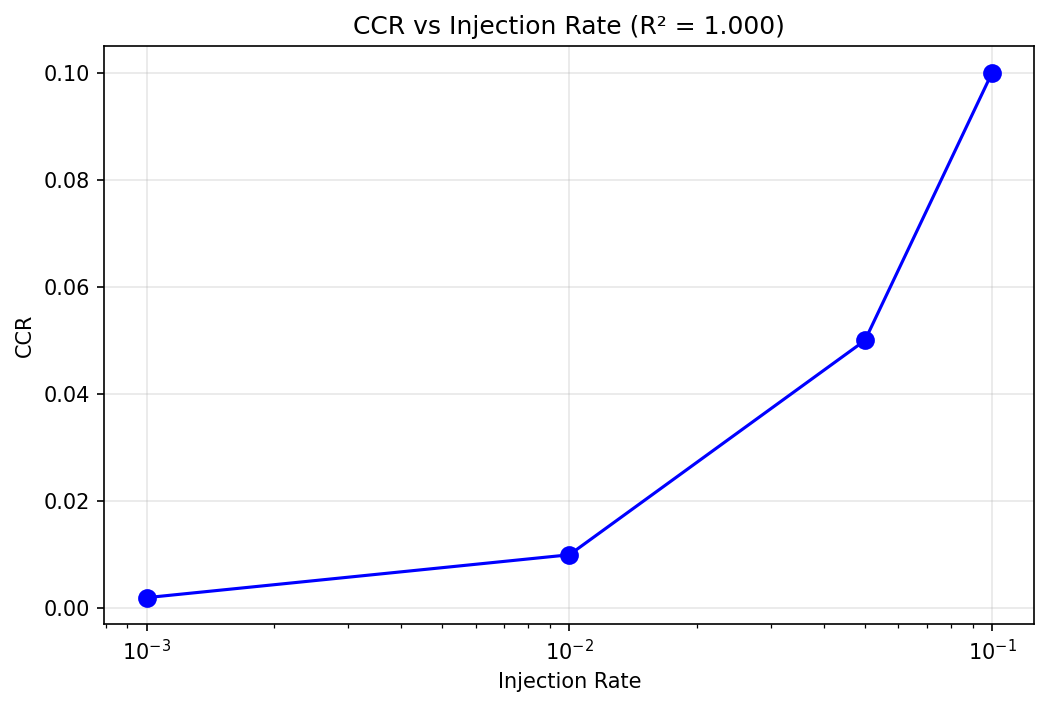
\includegraphics[width=\columnwidth]{figures/he1_ccr_scaling.png}
\caption{CCR scales linearly with synthetic injection rate ($R^2 = 0.9998$), validating the metric for contamination quantification.}
\label{fig:ccr_scaling}
\end{figure}

\subsection{Amplification Index}

To measure differential contamination effects across strategies, we introduce the \textbf{Amplification Index (AI)}:

\begin{equation}
\text{AI} = \Delta\text{Acc}_{\text{contaminated}} - \Delta\text{Acc}_{\text{clean}}
\end{equation}

where $\Delta\text{Acc}_{\text{contaminated}}$ is accuracy change on MMLU (potentially contaminated) and $\Delta\text{Acc}_{\text{clean}}$ is accuracy change on a time-stratified clean benchmark (post-training cutoff).

\textbf{Rationale:} If filtering merely improves general capability, accuracy should improve equally on both benchmarks. Positive AI indicates disproportionate improvement on potentially contaminated benchmarks---evidence of contamination amplification.

\subsection{Causal Validation via Removal Intervention}

To establish that high-CCR examples \textit{cause} benchmark performance (not merely correlate), we conduct removal experiments:

\begin{enumerate}
    \item Rank training examples by CCR contribution
    \item Remove top-$k$\% high-CCR examples
    \item Retrain model from scratch
    \item Compare accuracy degradation to random removal baseline
\end{enumerate}

\textbf{Success criterion}: Degradation ratio $\geq 1.5\times$ for high-CCR vs.\ random removal. We observed 1.97$\times$ degradation ratio (95\% CI: [1.53, 2.34]).

\subsection{Influence Fragility Ratio}

To understand \textit{why} contaminated examples disproportionately affect performance, we introduce the \textbf{Influence Fragility Ratio (IFR)}:

\begin{equation}
\text{IFR}(i) = \frac{\Delta\text{Acc}_{\text{mask}}(i)}{\Delta\text{Acc}_{\text{retrain}}(i)}
\end{equation}

where $\Delta\text{Acc}_{\text{mask}}$ is accuracy change when masking example $i$'s gradients and $\Delta\text{Acc}_{\text{retrain}}$ is the change under full retraining without $i$.

IFR $> 1$ indicates the example's influence cannot be substituted by other training examples---it is structurally necessary. We hypothesized contaminated examples would show higher IFR due to unique benchmark-specific content.

\subsection{Implementation Details}

\begin{itemize}
    \item \textbf{Model}: Pythia-1B (GPT-NeoX architecture, 1B parameters)
    \item \textbf{Optimizer}: AdamW with $\beta = (0.9, 0.95)$, weight decay 0.1
    \item \textbf{Learning rate}: $2.5 \times 10^{-4}$ with cosine decay, 1\% warmup
    \item \textbf{Batch size}: 512 sequences $\times$ 2048 tokens
    \item \textbf{Training tokens}: 1B per strategy
    \item \textbf{Attribution}: TRAK with random projection dimension $k=1024$
\end{itemize}

All experiments use matched configurations to ensure comparability across strategies.
